
A network both defines the composition advected by the hydro code
as well as describes the burning processes between those isotopes.

In this chapter on nuclear networks, we list the network routines
available for your use, and then we describe the correct structure of
a network module in case you want to build your own.

\section{Network List}

\subsection{{\tt general\_null}}

{\tt general\_null} is a bare interface for a nuclear reaction
network; no reactions are enabled, and no auxiliary variables are
accepted. It contains several sets of isotopes; for example, {\tt
  Networks/general\_null/triple\_alpha\_plus\_o.net} would describe
the triple-$\alpha$ reaction converting helium into carbon, as well as
oxygen and iron.

\subsection{{\tt ignition\_chamulak}}

This network was introduced in our paper on convection in white dwarfs
as a model of Type Ia supernovae~\cite{wdconvect}.  It models
carbon burning in a regime appropriate for a simmering white dwarf,
and captures the effects of a much larger network by setting the ash
state and energetics to the values suggested in \cite{chamulak:2008}.


\subsection{{\tt Networks/ignition\_simple}}

This is the original network used in our white dwarf convection
studies~\cite{lowMach4}.  It includes a single-step
$^{12}\mathrm{C}(^{12}\mathrm{C},\gamma)^{24}\mathrm{Mg}$ reaction.
The carbon mass fraction equation appears as
\begin{equation}
\frac{D X(^{12}\mathrm{C})}{Dt} = - \frac{1}{12} \rho X(^{12}\mathrm{C})^2
    f_\mathrm{Coul} \left [N_A \left <\sigma v \right > \right]\enskip,
\end{equation}
where $N_A \left <\sigma v\right>$ is evaluated using the reaction
rate from (Caughlan and Fowler 1988).  The Coulomb screening factor,
$f_\mathrm{Coul}$, is evaluated using the general routine from the
Kepler stellar evolution code (Weaver 1978), which implements the work
of (Graboske 1973) for weak screening and the work of (Alastuey 1978
and Itoh 1979) for strong screening.



\section{Network Structure}
\label{section:network_structure}

There are three primary files within each network directory.

{\tt actual\_network.f90} supplies the number and names of species and
auxiliary variables, as well as other initializing data, such as their
mass numbers, proton numbers, and binding energies. It needs to define
the {\tt nspec} and {\tt naux} quantities as integer parameters. Additionally
it must define {\tt nspec\_evolve}, the number of species that are actually evolved
during a burn; in most cases, this should have the same value as {\tt nspec}.
Finally, it must also define {\tt nrates}, the number of reaction rates
linking the isotopes in the network.

{\tt actual\_rhs.f90} supplies an interface for computing the right-hand-side
of the network, the time-derivative of each species (and the temperature and
nuclear energy release), as well as the Jacobian. This is covered in more detail
in Chapter \ref{chapter:burners}.

{\tt actual\_burner.f90} contains the interface for doing an actual burn.
In general, you will want to {\tt call integrator} to use one of the pre-defined
ODE integrators, but you could also write a custom integration here. This is
covered in more detail in Chapter \ref{chapter:burners}.

All three have initialization routines ({\tt actual\_network\_init()},
{\tt actual\_rhs\_init()}, and {\tt actual\_burner\_init()}) which must
be called upon initialization. These should be not called within
OpenMP parallel regions, because in general they will modify shared module data.



\begin{sidewaysfigure}
\centering
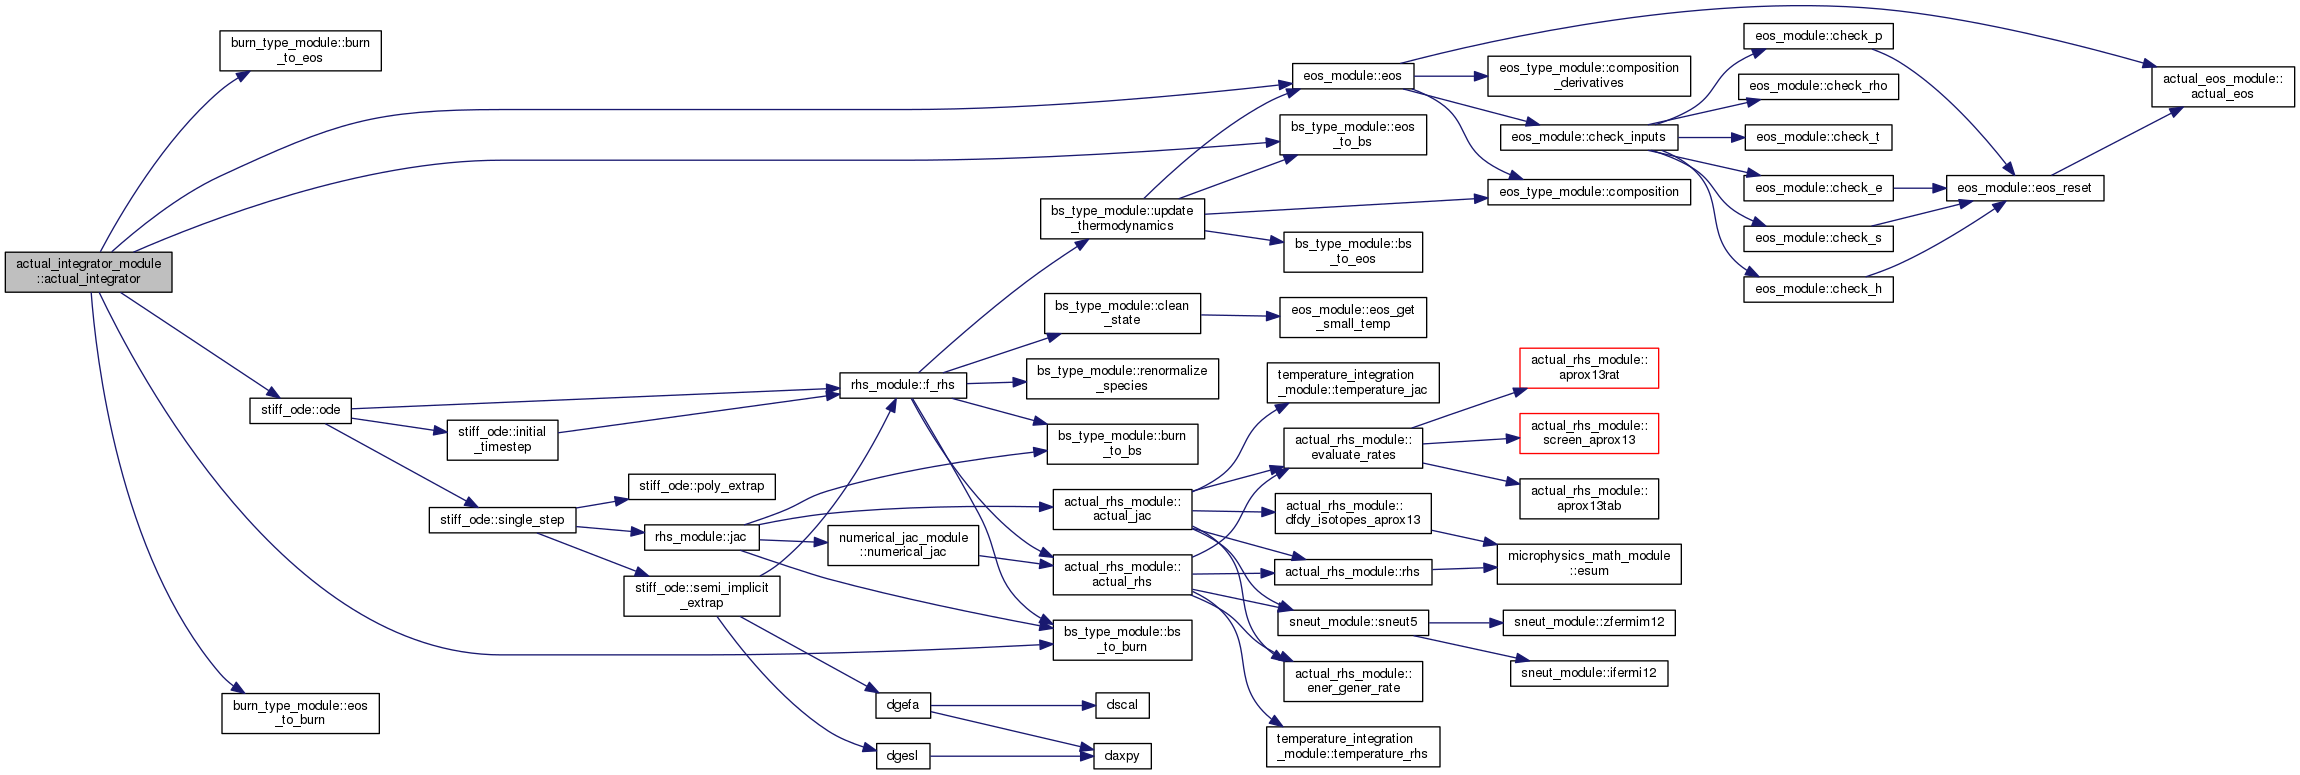
\includegraphics[width=\linewidth]{doxygen_network}
\end{sidewaysfigure}
